\documentclass[letterpaper,USenglish,cleveref, autoref, thm-restate]{lipics-v2021}
%This is a template for producing LIPIcs articles. 
%See lipics-v2021-authors-guidelines.pdf for further information.
%for A4 paper format use option "a4paper", for US-letter use option "letterpaper"
%for british hyphenation rules use option "UKenglish", for american hyphenation rules use option "USenglish"
%for section-numbered lemmas etc., use "numberwithinsect"
%for enabling cleveref support, use "cleveref"
%for enabling autoref support, use "autoref"
%for anonymousing the authors (e.g. for double-blind review), add "anonymous"
%for enabling thm-restate support, use "thm-restate"
%for enabling a two-column layout for the author/affilation part (only applicable for > 6 authors), use "authorcolumns"
%for producing a PDF according the PDF/A standard, add "pdfa"

%\pdfoutput=1 %uncomment to ensure pdflatex processing (mandatatory e.g. to submit to arXiv)
%\hideLIPIcs  %uncomment to remove references to LIPIcs series (logo, DOI, ...), e.g. when preparing a pre-final version to be uploaded to arXiv or another public repository

%\graphicspath{{./graphics/}}%helpful if your graphic files are in another directory

\usepackage{amsmath}
\usepackage{tikz}
\usepackage{pgfplots}
\usepackage{booktabs}

\newcommand{\pand}{\mathbin{\land^{\sf p}}}
\newcommand{\por}{\mathbin{\lor^{\sf p}}}
\DeclareMathOperator*{\Pand}{\bigwedge^{\sf v}}
\DeclareMathOperator*{\Por}{\bigvee^{\sf a}}
\newcommand{\boolnot}{\neg}
\newcommand{\tautology}{\top}
\newcommand{\nil}{\bot}
\newcommand{\obar}[1]{\overline{#1}}
\newcommand{\oneminus}{{\sim}}
\newcommand{\lit}{\ell}

\newcommand{\varset}{X}
\newcommand{\exvarset}{Z}
\newcommand{\dependencyset}{{\cal D}}
\newcommand{\litset}{{\cal L}}
\newcommand{\ring}{{\cal R}}
\newcommand{\dset}{{\cal A}}
\newcommand{\rep}{\textbf{R}}
\newcommand{\radd}{+}
\newcommand{\rmul}{\times}
\newcommand{\addident}{\textbf{0}}
\newcommand{\mulident}{\textbf{1}}
\newcommand{\imply}{\Rightarrow}

\newcommand{\assign}{\alpha}
\newcommand{\passign}{\rho}
\newcommand{\uassign}{{\cal U}}
\newcommand{\modelset}{{\cal M}}

\newcommand{\indegree}{\textrm{indegree}}
\newcommand{\outdegree}{\textrm{outdegree}}
\newcommand{\validate}{\textsf{validate}}

\newcommand{\simplify}[2]{#1|_{#2}}
\newcommand{\prov}{\mathit{Expand}}

\newcommand{\progname}[1]{\textsc{#1}}
\newcommand{\dfour}{\progname{d4}}
\newcommand{\Dfour}{\progname{d4}}
\newcommand{\generator}{\progname{d2p}}
\newcommand{\Generator}{\progname{d2p}}
\newcommand{\checker}{\progname{crat-check}}
\newcommand{\Checker}{\progname{Crat-check}}


\bibliographystyle{plainurl}% the mandatory bibstyle

\title{Certified Knowledge Compilation \\ with Application to Verified Model Counting}

\titlerunning{Certified Knowledge Compilation}

\author{Randal E. Bryant}{Computer Science Department, Carnegie Mellon University, Pittsburgh, PA 15213 USA}{rebryant@cmu.edu}{https://orcid.org/0000-0001-5024-6613}{Supported by NSF grant CCF-2108521}
\author{Wojciech Nawrocki}{Department of Philosophy, Carnegie Mellon University}{wjnawrock@cmu.edu}{https://orcid.org/0000-0002-8839-0618}{}
\author{Jeremy Avigad}{Department of Philosophy, Carnegie Mellon University}{avigad@cmu.edu}{https://orcid.org/0000-0003-1275-315X}{}
\author{Marijn J. H. Heule}{Computer Science Department, Carnegie Mellon University}{marijn@cmu.edu}{https://orcid.org/0000-0002-5587-8801}{Supported by NSF grant CCF-2108521}

\authorrunning{R. E. Bryant, et al} %TODO mandatory. First: Use abbreviated first/middle names. Second (only in severe cases): Use first author plus 'et al.'

%\Copyright{Jane Open Access and Joan R. Public} %TODO mandatory, please use full first names. LIPIcs license is "CC-BY";  http://creativecommons.org/licenses/by/3.0/

%\ccsdesc[100]{\textcolor{red}{Replace ccsdesc macro with valid one}} %TODO mandatory: Please choose ACM 2012 classifications from https://dl.acm.org/ccs/ccs_flat.cfm 

%\keywords{Dummy keyword} %TODO mandatory; please add comma-separated list of keywords

%\category{} %optional, e.g. invited paper

%\funding{(Optional) general funding statement \dots}%optional, to capture a funding statement, which applies to all authors. Please enter author specific funding statements as fifth argument of the \author macro.

%\nolinenumbers %uncomment to disable line numbering

%Editor-only macros:: begin (do not touch as author)%%%%%%%%%%%%%%%%%%%%%%%%%%%%%%%%%%
%\EventEditors{John Q. Open and Joan R. Access}
%\EventNoEds{2}
%\EventLongTitle{42nd Conference on Very Important Topics (CVIT 2016)}
%\EventShortTitle{CVIT 2016}
%\EventAcronym{CVIT}
%\EventYear{2016}
%\EventDate{December 24--27, 2016}
%\EventLocation{Little Whinging, United Kingdom}
%\EventLogo{}
%\SeriesVolume{42}
%\ArticleNo{23}
%%%%%%%%%%%%%%%%%%%%%%%%%%%%%%%%%%%%%%%%%%%%%%%%%%%%%%

\newcommand{\program}[1]{\textsc{#1}}
\newcommand{\lean}{\program{lean4}}

\begin{document}

\maketitle

\begin{abstract}
Knowledge compilers convert Boolean formulas into a form for which
useful tasks, including model counting and weighted model counting,
can easily be performed.  Existing knowledge compilers, however,
provide no guarantee that the generated representation accurately
describes the original formula.

We present the Partitioned Operation Graph (POG) representation that
generalizes existing knowledge compiler representations, and a proof
framework that can prove the equivalence of a POG representation with
a conjunctive normal form (CNF) Boolean formula.

We have developed a program that can generate POG representations and
equivalence proofs from the d-DNNF graphs generated by a leading
knowledge compiler.  It scales to all but the largest formulas from a
recent model counting competition.  We also present two proof
checkers---a fast checker that can handle the large proofs generated,
and a formally verified checker written in the \lean{} proof system.
\end{abstract}

\section{Introduction}

\begin{figure}
\centering{
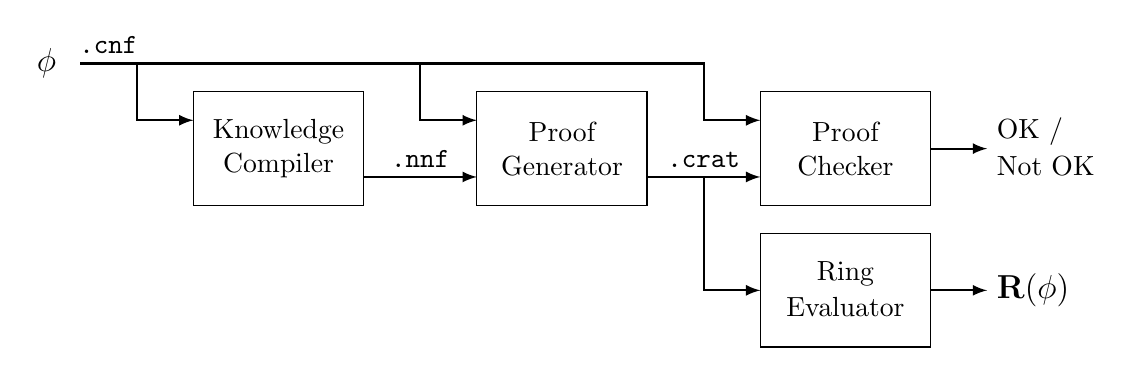
\begin{tikzpicture}[scale=0.18]
  \draw (8,10) rectangle (20,18);
  \node at (14,15.2) {Knowledge};
  \node at (14,12.8) {Compiler};

  \draw (28,10) rectangle (40,18);
  \node at (34,15.2) {Proof};
  \node at (34,12.8) {Generator};


  \draw (48,10) rectangle (60,18);
  \node at (54,15.2) {Proof};
  \node at (54,12.8) {Checker};

  \draw (48,0) rectangle (60,8);
  \node at (54,5.2) {Ring};
  \node at (54,2.8) {Evaluator};


  %% CNF
  \draw[thick] (0,20) -- (44,20) -- (44,16) [-latex] -- (48,16);
  \draw[thick] (4,20) -- (4,16) [-latex] -- (8,16);
  \draw[thick] (24,20) -- (24,16) [-latex] -- (28,16);
  \node [left] at (-1,20) {\large {$\phi$}};
  \node [above] at (2,20) {\texttt{.cnf}};

  %% NNF
  \draw[thick] (20,12) [-latex] -- (28,12);
  \node [above] at (24,12) {\texttt{.nnf}};

  %% CRAT
  \draw[thick] (40,12) [-latex] -- (48,12);
  \draw[thick] (44,12) -- (44,4) [-latex] -- (48,4);
  \node [above] at (44,12) {\texttt{.crat}};

  %% OK/Not
  \draw[thick] (60,14) [-latex] -- (64,14) ;
  \node [right] at (64,15.2) { OK /} ;
  \node [right] at (64,12.8) { Not OK} ;
  \draw[thick] (60,4) [-latex] -- (64,4) ;
  \node [right] at (64,4) {\large {$\textbf{R}(\phi)$}};

\end{tikzpicture}
}
\caption{Tool Chain. The output of a standard knowledge compiler is converted into a combined graph/proof (CRAT) that can be independently checked and evaluated}
\label{fig:chain}
\end{figure}

\section{Logical Foundations}

  Let $\varset$ denote a set of Boolean variables, and let $\assign$
  be an {\em assignment} of truth values to some subset of the
  variables, where $0$ denotes false and $1$ denotes true, i.e.,
  $\assign \colon \varset' \rightarrow \{0,1\}$ for some $\varset'
  \subseteq \varset$.  We say the assignment is {\em total} when it
  assigns a value to every variable ($\varset' = \varset$), and that
  it is {\em partial} otherwise.
  The set of all possible total assignments over
  $\varset$ is denoted $\uassign$.

For each variable $x \in \varset$,
  we define {\em literals} $x$ and $\obar{x}$, where $\obar{x}$ is the
  negation of $x$. An
  assignment $\assign$ can be viewed as a set of literals, where
  we write $\lit \in \assign$ when $\lit = x$ and $\assign(x) = 1$ or when
  $\lit = \obar{x}$ and $\assign(x) = 0$.  We write the negation of literal $\lit$ as $\obar{\lit}$.  That is, $\obar{\lit} = \obar{x}$ when $\lit = x$ and
$\obar{\lit} = x$ when $\lit = \obar{x}$.


\begin{definition}[Boolean Formulas]
  The set of Boolean formulas is defined recursively.  Each
  formula $\phi$ has an associated {\em dependency set}
  $\dependencyset(\phi)  \subseteq \varset$, and a set of models $\modelset(\phi)$,
  consisting of total assignments that satisfy the formula:
  \begin{enumerate}
  \item Boolean constants $0$ and $1$ are Boolean formulas,
    with $\dependencyset(0) = \dependencyset(1) = \emptyset$, with $\modelset(0) = \emptyset$, and with $\modelset(1) = \uassign$.
  \item Variable $x$ is a Boolean formula, with $\dependencyset(x) = \{x\}$
    and $\modelset(x) = \{\assign \in \uassign | \assign(x)=1\}$.
  \item For formula $\phi$, its {\em negation}, written $\boolnot \phi$ is a Boolean formula,
    with $\dependencyset(\boolnot \phi) = \dependencyset(\phi)$ and $\modelset(\boolnot \phi) = \uassign - \modelset(\phi)$.
  \item For formulas $\phi_1, \phi_2, \ldots, \phi_k$, their {\em conjunction} $\phi = \bigwedge_{i=1,k} \phi_i$ is a Boolean formula, with
      $\dependencyset(\phi) = \bigcup_{i=1,k} \dependencyset(\phi_i)$ and
      $\modelset(\phi) = \bigcap_{i=1,k} \modelset(\phi_i)$.
  \item For formulas $\phi_1, \phi_2, \ldots, \phi_k$, their {\em disjunction} $\phi = \bigvee_{i=1,k} \phi_i$ is a Boolean formula, with
      $\dependencyset(\phi) = \bigcup_{i=1,k} \dependencyset(\phi_i)$ and
      $\modelset(\phi) = \bigcup_{i=1,k} \modelset(\phi_i)$.
  \end{enumerate}
\label{def:boolean}
\end{definition}
  
  We highlight the following special classes of Boolean formulas:
  \begin{description}
    \item[Normal form:] A formula where negation is applied only to variables.
    \item[Conjunctive Normal Form (CNF):] A normal form formula where  disjunction is applied only to literals.
    \item[Partitioned-Operation:] A formula satisfying the following for all conjunction and disjunction operations: 
      \begin{itemize}
      \item The arguments to a conjunction must have disjoint dependency sets.  That is, operation
        $\bigwedge_{i=1,k} \phi_i$ requires $\dependencyset(\phi_i) \cap \dependencyset(\phi_j) = \emptyset$ for $1 \leq i < j \leq k$.
      \item The arguments to a disjunction must have disjoint models.  That is, operation
        $\bigvee_{i=1,k} \phi_i$ requires $\modelset(\phi_i) \cap \modelset(\phi_j) = \emptyset$ for $1 \leq i < j \leq k$.
      \end{itemize}
  \end{description}
     We let $\pand$ and $\por$ denote the conjunction and disjunction operations in a partitioned-operation formula.
     A formula in conjunctive normal form can be represented by a set
     of {\em clauses}, each of which is a set of literals.  Each
     clause then represents the disjunction of the literals, and the formula is then the conjunction of its clauses.
  
  \section{Ring Evaluation of a Boolean Formula}

We propose a general framework for 
summarizing properties of Boolean formulas.

\begin{definition}[Commutative Ring]
  A {\em commutative ring} $\ring$ is an algebraic structure
  $\langle \dset, \radd, \rmul, \addident, \mulident \rangle$, 
  with elements in the set $\dset$ and with commutative and
  associative operations $\radd$ (addition) and $\rmul$ (multiplication),
  such that multiplication distributes
  over addition.  $\addident$ is the additive identity and $\mulident$ is
  the multiplicative identity.  Every element $a \in \dset$ has an
  {\em additive inverse} $-a$ such that $a + -a = \addident$.
\label{def:ring}
\end{definition}
We write $a - b$ as a shorthand for $a + -b$.

\begin{definition}[Ring Evaluation Problem (REP)]
  For ring $\ring$, a {\em ring labeling} associates a value $w(x) \in \dset$ with
  every variable $x \in \varset$.  We then define $w(\obar{x})$ to equal $1-w(x)$.

  For Boolean formula $\phi$, the {\em ring evaluation problem} (REP) is to compute:
  \begin{eqnarray}
    \rep(\phi) & = & \sum_{\alpha \in \modelset(\phi)} \;\; \prod_{\lit \in \alpha} w(\ell) \label{eqn:rep}
  \end{eqnarray}
\label{def:labeling}
\end{definition}

A wide variety of important tasks for Boolean functions can be
expressed as ring evaluation problems.  The 
{\em model counting} problem for formula $\phi$ requires determining $|\modelset(\phi)|$
It can be cast as an REP by having $\radd$ and
$\rmul$ be addition and multiplication over rational numbers and using
label $w(x) = 1/2$ for every variable $x$.  
Ring evaluation of formula $\phi$ will then compute the {\em density} of
the formula, i.e., the fraction of all possible total assignments that are
models.  For $n = |\varset|$, scaling the density by $2^n$ will then
yield the number of models.

The {\em weighted model counting} (WMC) problem is also defined over
rational numbers.  Some formulations of WMC allow 
assigning weights $W$ to both the variables and their negations, such
that there can be variables $x$ with $W(x) + W(\obar{x}) \not = 1$.  We can convert this more general form into a
ring evaluation problem by letting $r(x) = W(x) + W(\obar{x})$,
performing ring evaluation with label $w(x) = W(x)/r(x)$ for each
variable $x$, and then computing the final result as $\rep(\phi)\;
\rmul\; \prod_{x \in \varset} r(x)$.  Of course, this requires that $r(x) \not = 0$ for all $x \in \varset$.

The {\em function hashing problem} provides a randomized test
of inequivalence for Boolean formulas.  That is, for $n = |\varset|$, let $\ring$ be a
finite  field with $|\dset| = m$ such that $m \geq 2 n$.  For each $x \in \varset$, chose a value from $\dset$ at random for $w(x)$.  Two formulas
$\phi_1$ and $\phi_2$ will clearly have $\rep(\phi_1) = \rep(\phi_2)$
if they are logically equivalent.  If they are not equivalent, then
the probability that $\rep(\phi_1) \not = \rep(\phi_2)$ will be at
least $\left(1-\frac{1}{m}\right)^n \geq \left(1-\frac{1}{2n}\right)^n > 1/2$.
Therefore, ring evaluation can be used as part of a
randomized algorithm for equivalence testing~\cite{blum:ipl:1980}.

Possible generalizations of this framework are discussed in Section~\ref{sect:future}.

\section{Partitioned-Operation Graphs (POGs)}

Performing ring evaluation on an arbitrary Boolean formula could be intractable, but it is straightforward for a formula with partitioned operations:
\begin{proposition}
Ring evaluation with operations $\boolnot$, $\pand$, and $\por$ satisfies the following:
\begin{description}
\item[Negation] $\rep(\boolnot \phi) = \mulident - \rep(\phi)$
\item[Partitioned Conjunction] $\rep\left(\Pand_{i=1,k} \phi_i\right) = \prod_{i=1,k} \rep(\phi_i)$
\item[Partitioned Disjunction] $\rep\left(\Por_{i=1,k} \phi_i\right) = \sum_{i=1,k} \rep(\phi_i)$
\end{description}
\end{proposition}

A {\em partitioned-operation graph} (POG) is a directed, acyclic graph
with nodes $N$ and edges $E \subseteq N \times N$.  When $(u,v) \in E$,
node $v$ is said to be a {\em child} of node $u$.
The in- and out-degrees of node $u$ are defined as $\indegree(u) = | E \cap (N \times \{u\}) |$, and
$\outdegree(u) = | E \cap (\{u\} \times N) |$.
Node $u$ is said to be {\em terminal} if $\outdegree(u) = 0$.  A terminal node is labeled by a Boolean constant or variable.
Node $u$ is said to be {\em nonterminal} if $\outdegree(u) > 0$.  A nonterminal node is labeled by one of three Boolean operations:
$\boolnot$, $\pand$, or $\por$.  Node $u$ can be labeled with $\boolnot$ only if $\outdegree(u) = 1$.
It can be labeled with operation $\pand$ or $\por$ only if it satisfies the partitioning restriction for that operation.
There is a unique {\em root node} $r$ such that $\indegree(r) = 0$.

As can be seen, a POG is simply a way to represent a partitioned-operation
formula with a sharing of common subformulas.  Indeed, every node the graph can be viewed as a partitioned-operation formula, and so we write
$\phi(u)$ as the formula denoted by node $u$ and write $\phi(P) = \phi(r)$ for root $r$ of $P$.

We define the {\em size} of POG $P$, written $|P|$ to be the sum of
the number of nonterminal nodes and the number of edges.  Ring
evaluation of $\phi(P)$ can be performed with at most $|P|$ ring
operations by traversing the graph from the terminal nodes up to
the root, computing a value $\rep(u)$ for each node $u$.

POGs are inspired by the d-DNNF graphs devised by Darwiche for
representing Boolean functions \cite{darwiche:jair:2002}.
POGs generalize d-DNNF in two ways:
\begin{itemize}
\item They allow negation of arbitrary nodes in the graph, not just
  variables.  As we have seen, ring evaluation can readily handle negation, and so we allow it in the interest of generality.
  Negation could be useful in some contexts, such as when
  converting binary decision diagrams (BDDs) having complemented
  edges~\cite{brace-dac-1990,minato-dac-1990} into POGs.

\item They allow arbitrary arguments to a $\por$ operation, as long as
  they have disjoint models.  By contrast, each
  disjunction node $v$ in a d-DNNF can have at most two children $u_1$ and $u_0$ for which there must be a {\em splitting variable} $x$ such that
  any total assignment $\assign$ satisfying $\phi(u_1)$ has $\assign(x)=1$, while any total assignment satisfying $\phi(u_0)$ has
  $\assign(x)=0$.  Our generalization is provided to allow an
  encoding of Sentential Decision Diagrams (SDDs)~\cite{darwiche:ijcai:2011} into
  POGs.  This is discussed in Section~\ref{sect:future}, describing possible future research.
\end{itemize}
  Both of these generalizations allow more flexibility in the POG
  representation while maintaining the ability to efficiently perform ring evaluation.


\section{The CRAT POG Representation and Proof System}

A CRAT file provides both a declaration of a POG, as well as a checkable, clausal
proof that a Boolean formula, given in conjunctive normal
form, is logically equivalent to the POG, thus enabling certified
knowledge compilation.  The proof system is based on extended
resolution~\cite{Tseitin:1983} with reverse unit propagation
(RUP)~\cite{goldberg,vangelder08_verifying_rup_proofs} as the core method for
proving that a set of clauses logically implies another clause.

As is shown in Figure~\ref{fig:chain}
two programs are involved in producing a certified compilation of a formula:
\begin{itemize}
\item The {\em proof generator} generates a CRAT file that both describes a POG and provides a proof that this POG is equivalent to the input formula.
  This compiler might start with the output of another knowledge compiler.
\item The {\em proof checker} ensures that all of the proof conditions are satisfied.  
\end{itemize}

The CRAT format draws its inspiration from the LRAT format for Boolean
formulas~\cite{lrat} and the QRAT format for quantified Boolean
formulas (QBF)~\cite{heule:JAR2014}.  The following are its key properties:
\begin{itemize}
  \item
  The file contains declarations of $\pand$ and $\por$ operations to describe the POG.
  Each such declaration implicitly adds an extension variable representing the POG node and a set of {\em defining} clauses
  encoding the conjunction or disjunction operation.
  This is the only means for adding extension variables to the proof.
\item Boolean negation is supported implicitly by allowing the
  arguments of the $\por$ and $\pand$ operations to be literals and not just
  variables.
\item
  The file contains explicit clause addition steps.
  A clause can only be added if it is logically implied by the existing clauses.
  A sequence of clause identifiers must be listed as {\em hints} providing a RUP verification of the implication.
\item
  The file contains explicit clause deletion steps.
  A clause can only be deleted if it is logically implied by the remaining clauses.
  A sequence of clause identifiers must be listed as {\em hints} providing a RUP verification of the implication.
\item The checker must track the dependency set for every input and
  extension variable.  For each $\pand$ operation, the checker must ensure that the dependency sets for its arguments are disjoint.
  The associated extension variable has a dependency set equal to the union of those of its arguments.
\item Declaring a $\por$ operation requires a sequence of clauses
  providing a RUP proof that the arguments are mutually exclusive.
  Only binary $\por$ operations are allowed to avoid requiring
  $k\,(k-1)/2$ proofs of disjointness for larger values of $k$.
\end{itemize}

\subsection{Syntax}

\begin{table}
  \caption{CRAT Step Types.  $C$: clause identifier, $L$: literal, $V$: variable}
  \label{tab:crat:syntax}
\centering{
  \begin{tabular}{lllll}
    \multicolumn{4}{c}{Rule} & \multicolumn{1}{c}{Description} \\
    \midrule
    \makebox[5mm][l]{$C$} & \makebox[10mm][l]{\tt a}  & \makebox[15mm][l]{$L^{*}$ {\tt 0}} & \makebox[15mm][l]{$C^{+}$ {\tt 0}}  & \makebox[20mm][l]{Add RUP clause} \\
     & {\tt dc} & $C$             & $C^{+}$  {\tt 0} & Delete RUP clause \\
    \midrule
    $C$    & {\tt p} & $V \; L^{*}$ {\tt 0}    &                  & Declare $\pand$ operation \\
    $C$    & {\tt s} & $V \; L \; L$    & $C^{+}$ {\tt 0}  & Declare $\por$ operation \\ 
    \midrule
     & {\tt r} & $L$             &            & Declare root literal\\
  \end{tabular}
  }
\end{table}

Table~\ref{tab:crat:syntax} shows the declarations that can occur in a CRAT file.
The checker is provided with the input formula as a separate file.
As with other clausal proof formats, a variable is
represented by a positive integer $v$, with the first ones being input
variables and successive ones being extension variables.  Literal $\lit$
is represented by a signed integer, with $-v$ being the complement of
variable $v$.  Each clause is indicated by a positive integer
identifier $C$, with the first ones being the IDs of the input clauses and successive
ones being the IDs of added clauses.  Clause identifiers must be totally ordered,
such that clause $C$ can only reference clauses $C'$ such that $C' < C$.

The first set of proof rules are similar to those in other clausal
proofs.
Clauses can be added via RUP addition
(command {\tt a}), with a sequence of antecedent clauses (the
``hint'').
Similarly for clause deletion (command {\tt dc}).

The declaration of a $\pand$ operation has the form:
\begin{center}
\begin{tabular}{ccccccccc}
  \makebox[5mm]{$i$} & \makebox[5mm]{{\tt p}} & \makebox[5mm]{$v$} & \makebox[5mm]{$\lit_1$} & \makebox[5mm]{$\lit_2$} &
  \makebox[5mm]{$\cdots$} & \makebox[5mm]{$\lit_k$} & \makebox[5mm]{\tt 0} \\
\end{tabular}
\end{center}
where $i$ is a new clause ID, $v$ is a positive integer that does not
correspond to any previous variable, and $\lit_1, \lit_2, \ldots, \lit_k$ is a sequence of $k$  
integers representing literals of existing variables.  
This declaration implicitly causes $k+1$ clauses to be added to the proof:
\begin{center}
\begin{tabular}{cccccc}
\makebox[10mm]{ID} & \multicolumn{5}{c}{Clause} \\
  $i$ & $v$ & $-\lit_1$ & $-\lit_2$ & $\cdots$ & $-\lit_k$\\
  $i\!+\!1$ & $-v$ & $\lit_1$  \\
  $i\!+\!2$ & $-v$ & $\lit_2$  \\
  & $\ldots$ \\
  $i\!+\!k$ & $-v$ & $\lit_k$  \\
\end{tabular}
\end{center}
The dependency sets for the arguments represented by each pair of
literals $\lit_i$
and $\lit_{j}$ must
be disjoint, for $1 \leq i < j \leq k$.  A $\pand$ operation may have no arguments,
representing Boolean constant $1$.  The only clause added to the proof will be
the unit literal $v$.  A reference to literal $-v$ then becomes a way
of representing constant $0$.


The declaration of a $\por$ operation has the form:
\begin{center}
\begin{tabular}{ccccccc}
  \makebox[5mm]{$i$} & \makebox[5mm]{{\tt s}} & \makebox[5mm]{$v$} & \makebox[5mm]{$\lit_1$} & \makebox[5mm]{$\lit_2$} 
\makebox[5mm]{$H$} & \makebox[5mm]{$\texttt{0}$} \\
\end{tabular}
\end{center}
where $i$ is a new clause ID, $v$ is a positive integer that does
not correspond to any previous variable, and $\lit_1$ and $\lit_2$ are
signed integers representing literals of existing variables.  Hint $H$
consists of a
sequence of clause IDs.
This declaration implicitly causes three clauses to be added to the proof:
\begin{center}
\begin{tabular}{cccc}
\makebox[10mm]{ID} & \multicolumn{3}{c}{Clause} \\
  $i$ & $-v$ & $\lit_1$ & $\lit_2$ \\
  $i\!+\!1$ & $v$ & $-\lit_1$ \\
  $i\!+\!2$ & $v$ & $-\lit_2$ \\
\end{tabular}
\end{center}
The hints must provide a RUP proof of the clause $\obar{\lit}_1 \lor \obar{\lit}_2$.

Finally, the literal denoting the root of the POG is declared with the
{\tt r} command.  It can occur anywhere in the file.  Typically, it
will be the extension variable representing the root of a graph, but in
degenerate cases it can be the positive or negative literal of an
input variable.

\subsection{Semantics}

Observe that the defining clauses for the conjunction and disjunction
operations provide a full Tseitin encoding of the operations.  Letting
$\exvarset$ denote the set of added extension variables,  any
total assignment $\assign\colon \varset \rightarrow \{0,1\}$ has a unique extension,
which we also call $\assign$, with $\assign\colon (\varset \cup \exvarset) \rightarrow \{0,1\}$.

A CRAT proof follows the same general form as a QRAT dual
proof~\cite{bryant:cade:2021}---one that ensures that each clause
addition and each clause deletion preserves equivalence.  With CRAT,
however, clauses are defined both explicitly and implicitly.  Starting
with the set of input clauses, the proof consists of a sequence of
steps that both add and delete clauses.  Each addition must be truth
preserving, that is, any satisfying total assignment for the set of clauses
before clause addition should still be a satisfying assignment afterwards.
Each deletion must be falsehood preserving.  That is, there can be no
new satisfying assignments when the clause is deleted.

At the completion of the proof, the following conditions must hold:
\begin{itemize}
\item All of the input clauses have been deleted.
\item There should be exactly one clause left that was added via RUP
  addition, and this should be a unit clause consisting of the root literal $r$.
\end{itemize}
The sequence of clause addition steps provide a proof that any
total assignment $\assign$ to the input variables that satisfies all of the
clauses must, when extended, assign $\assign(r) = 1$.  Conversely,
each proof step that deletes an input clause proves that any
total assignment $\alpha$ that falsifies the clause must, when extended,
assign $\assign(r) = 0$.

The sequence of operator declarations, asserted clauses, and deleted
clauses represents a systematic transformation of the input formula
into a POG\@.  Validating each of these steps serves to prove that the
POG is logically equivalent to the input formula.

\subsection{CRAT Example}

\begin{figure}
\begin{minipage}{0.62\textwidth}
(A)  Input Formula\\[1.2ex]
\begin{tabular}{lll}
\toprule
\makebox[5mm]{ID} & \makebox[15mm]{Clauses} & \\
\midrule
1 & \texttt{-1 3 -4} & \texttt{0} \\
2 & \texttt{-1 -3 4} & \texttt{0} \\
3 & \texttt{3 -4} & \texttt{0}\\
4 & \texttt{1 -3 4} & \texttt{0} \\
5 & \texttt{-1 -2} & \texttt{0} \\
\bottomrule
\end{tabular}
\\[1.8ex]
(C) POG Declaration\\[1.2ex]
\begin{tabular}{llll}
\toprule
\makebox[5mm]{ID} & \multicolumn{2}{l}{CRAT line} & Explanation \\
\midrule
6 & \texttt{p 5 -3 -4} & \texttt{0} & $p_5 = \obar{x}_3 \pand \obar{x}_4$ \\
9 & \texttt{p 6 3 4} & \texttt{0} & $p_6 = x_3 \pand x_4$ \\
12 & \texttt{s 7 5 6 7 10} & \texttt{0} & $s_7 = p_5 \por p_6$ \\
15 & \texttt{p 8 -1 7} & \texttt{0} & $p_8 = \obar{x}_1 \pand s_7$ \\ 
18 & \texttt{p 9 1 -2 7} & \texttt{0} & $p_9 = x_1 \pand \obar{x}_2 \pand s_7$ \\
22 & \texttt{s 10 8 9 16 19} & \texttt{0} & $s_{10} = p_8 \por p_9$ \\
 & \texttt{r 10} && Root $r = s_{10}$\\
\bottomrule
\end{tabular}
\end{minipage}
\begin{minipage}{0.35\textwidth}
(B) POG Representation \\
\input{dd/eg4}
\end{minipage}
%% Break
\\[2.5ex]
\begin{minipage}{0.45\textwidth}
(D) Implicit Clauses\\[1.2ex]
\begin{tabular}{llll}
\toprule
\makebox[5mm]{ID} & \multicolumn{2}{l}{Clauses} & Explanation \\
\midrule
\texttt{6} & \texttt{5 3 4} & \texttt{0} & Define $p_5$ \\
\texttt{7} & \texttt{-5 -3} & \texttt{0} & \\
\texttt{8} & \texttt{-5 -4} & \texttt{0} & \\
\midrule
\texttt{9} & \texttt{6 -3 -4} & \texttt{0} & Define $p_6$ \\
\texttt{10} & \texttt{-6 3} & \texttt{0} & \\
\texttt{11} & \texttt{-6 4} & \texttt{0} & \\
\midrule
\texttt{12} & \texttt{-7 5 6} & \texttt{0} & Define $s_7$ \\
\texttt{13} & \texttt{7 -5} & \texttt{0} & \\
\texttt{14} & \texttt{7 -6} & \texttt{0} & \\
\midrule
\texttt{15} & \texttt{8 1 -7} & \texttt{0} & Define $p_8$ \\
\texttt{16} & \texttt{-8 -1} & \texttt{0} & \\
\texttt{17} & \texttt{-8 7} & \texttt{0} & \\
\midrule
\texttt{18} & \texttt{9 -1 2 -7} & \texttt{0} & Define $p_9$ \\
\texttt{19} & \texttt{-9 1} & \texttt{0} & \\
\texttt{20} & \texttt{-9 -2} & \texttt{0} & \\
\texttt{21} & \texttt{-9 7} & \texttt{0} & \\
\midrule
\texttt{22} & \texttt{-10 8 9} & \texttt{0} & Define $s_{10}$ \\
\texttt{23} & \texttt{10 -8} & \texttt{0} & \\
\texttt{24} & \texttt{10 -9} & \texttt{0} & \\
\bottomrule
\end{tabular}
\end{minipage}
\begin{minipage}{0.49\textwidth}
(E) CRAT Assertions\\[1.2ex]
\begin{tabular}{llllll}
\toprule
\makebox[5mm]{ID} & \multicolumn{2}{l}{Clause} & \multicolumn{2}{l}{Hints} & Explanation \\
\midrule
\texttt{25} & \texttt{a 5 1 3} & \texttt{0} & \texttt{3 6} & \texttt{0} & $\obar{x}_1 \land \obar{x}_3 \imply p_5$ \\
\texttt{26} & \texttt{a 6 1 -3} & \texttt{0} & \texttt{4 9} & \texttt{0} & $\obar{x}_1 \land x_3 \imply p_6$ \\
\texttt{27} & \texttt{a 3 7 1} & \texttt{0} & \texttt{13 25} & \texttt{0} & $\obar{x}_3 \land \obar{x}_1 \imply s_7$  \\
\texttt{28} & \texttt{a 7 1} & \texttt{0} & \texttt{27 14 26} & \texttt{0} & $\obar{x}_1 \imply s_7$  \\
\texttt{29} & \texttt{a 8 1} & \texttt{0} & \texttt{28 15} & \texttt{0} & $\obar{x}_1 \imply p_8$  \\
\texttt{30} & \texttt{a 5 -1 3} & \texttt{0} & \texttt{1 6} & \texttt{0} & $x_1 \land \obar{x}_3 \imply p_5$ \\
\texttt{31} & \texttt{a 6 -1 -3} & \texttt{0} & \texttt{2 9} & \texttt{0} & $x_1 \land x_3 \imply p_6$ \\
\texttt{32} & \texttt{a 3 7 -1} & \texttt{0} & \texttt{13 30} & \texttt{0} & $\obar{x}_3 \land x_1 \imply s_7$  \\
\texttt{33} & \texttt{a 7 -1} & \texttt{0} & \texttt{32 14 31} & \texttt{0} & $x_1 \imply s_7$  \\
\texttt{34} & \texttt{a 9 -1} & \texttt{0} & \texttt{5 33 18} & \texttt{0} & $x_1 \imply p_9$  \\
\texttt{35} & \texttt{a 1 10} & \texttt{0} & \texttt{23 29} & \texttt{0} & $\obar{x}_1 \imply s_{10}$  \\
\texttt{36} & \texttt{a 10} & \texttt{0} & \texttt{35 24 34} & \texttt{0} & $s_{10}$ \\
\bottomrule
\end{tabular}
\\[1.5ex]
(F) Input Clause Deletions\\[1.2ex]
\begin{tabular}{lllll}
  \toprule
 \multicolumn{3}{l}{CRAT line} & Explanation\\
\midrule
 \texttt{dc 1} & \texttt{36 8 10 12 16 21 22} & \texttt{0} & Delete clause 1 \\
 \texttt{dc 2} & \texttt{36 7 11 12 16 21 22} & \texttt{0} & Delete clause 2 \\
 \texttt{dc 3} & \texttt{36 8 10 12 17 19 22} & \texttt{0} & Delete clause 3 \\
 \texttt{dc 4} & \texttt{36 7 11 12 17 19 22} & \texttt{0} & Delete clause 4 \\
 \texttt{dc 5} & \texttt{36 16 20 22} & \texttt{0} &  Delete clause 5 \\
\bottomrule
\end{tabular}
\end{minipage}
\caption{Example formula (A), its POG representation (B), and its CRAT proof (C)--(F)}
\label{fig:eg4:all}
\end{figure}

Figure \ref{fig:eg4:all} illustrates an example formula and shows how
the CRAT file declares its POG representation.  The input formula (A)
consists of five clauses over variables $x_1$, $x_2$, $x_3$, and
$x_4$.  The generated POG (B) has six nonterminal nodes representing four
conjunctions and two disjunctions.  We name these by the node type (product or sum) and the extension variable.
The first part of the CRAT file
(C) declares these nodes using clause IDs that increment by three or
four, depending on whether the node has two children or three.
The last two nonzero values in the sum declarations are hints providing the required mutual exclusion proof.

We step through a detailed example to provide a better understanding of the CRAT proof framework.
Figure
\ref{fig:eg4:all}(D) shows the defining clauses that are implicitly
defined by the POG operation declarations.  These do not appear in the
CRAT file.  Referring back to the declarations of the sum nodes in
Figure \ref{fig:eg4:all}, we can see that the declaration of node
$s_7$ had clause IDs 7 and 10 as hints.  We can see in Figure
\ref{fig:eg4:all}(A) that these two clauses resolve to the clause
$\obar{p}_5 \lor \obar{p}_6$, showing that the two children of $s_7$
have disjoint models.  Similarly, node $s_{10}$ is declared as having
clause IDs 16 and 19 as hints.  These resolve to the clause
$\obar{p}_8 \lor \obar{p}_9$, showing that the two children of
$s_{10}$ have disjoint models.

Figure \ref{fig:eg4:all}(E) provides the sequence of assertions
leading to unit clause 36, consisting of the literal $s_{10}$.  This clause indicates that $s_{10}$ is implied by the input clauses, i.e.,
any total assignment $\assign$
satisfying the input clauses must extend to one with $\assign(s_{10}) = 1$.
Working backward, we can see that
clause 29 indicates that node $p_8$ will be implied by the input
clauses when $\assign(x_1) = 0$, while clause 34 indicates that node $p_9$ will
be implied by the input clauses when $\assign(x_1) = 1$.  These serve as the
hints for clause 36.

Figure \ref{fig:eg4:all}(F) shows the RUP proof steps required to
delete the input clauses.  Consider the first of these, deleting
input clause $\obar{x}_1 \lor x_3 \lor \obar{x}_4$.  The requirement is to show
that there is no total assignment $\assign$ that falsifies this clause, but assigns $\assign(s_{10}) = 1$.
proof proceeds by first assuming that the clause is false, requiring
$\assign(x_1) = 1$, $\assign(x_3) = 0$, and $\assign(x_4) = 1$.  The hints then consist of unit
clauses (e.g., clause 36 asserting that $\alpha(p_{10}) = 1$) or
clauses that cause unit propagation.  Hint clauses 8 and 10 force the
assignments $\assign(p_5) = \assign(p_6) = 0$.  These, plus hint clause 12 forces
$\assign(s_7) = 0$.  This, plus hint clauses 16 and 21 force $\assign(p_8) = \assign(p_9) = 0$, leading
via clause 22 to $\assign(s_{10}) = 0$.  But this contradicts clause 22,
completing the RUP proof.  The deletion hints for the other input
clauses follow similar patterns---they work from the bottom nodes of
the POG upward, showing that any total assignment that falsifies the clause
must assign $s_{10} = 0$.

Deleting the asserted clauses so simple that we do not show it.  It
involves simply deleting the clauses from clause number 35 down to
clause number 25, with each deletion using the same hints as were used
to add that clause.  In the end, therefore, only the defining clauses
for the POG nodes and the unit clause asserting $s_{10}$ remain,
completing a proof that the POG is logically equivalent to the input
formula.

Observe that this proof must ``visit'' nodes
$p_5$ and $p_6$ twice, separately considering total assignments where $\assign(x_1) = 0$
(clauses 25 and 26) and where $\assign(x_1) = 1$ (clauses 30 and 31).  In
general, a naive proof must expand the POG into a tree.
We address this shortcoming by introducing {\em lemmas}, as is described in Section~\ref{sect:lemma}



\section{Generating CRAT from d-DNNF}

Figure~\ref{fig:chain} illustrates one method of generating a CRAT
file from an input formula in conjunctive normal form.  Our tool chain
is based on the \dfour{} knowledge compiler~\cite{lagniez:ijcai:2017},
but it would also work for other tools that use a top-down search
strategy to generate a d-DDNNF representation.  Converting a d-DNNF
graph into a POG is straightforward, each node in a d-DNNF graph can
be directly represented as a POG node.  We perform simplifications on
the d-DNNF representation to eliminate any Boolean constants.  We can
therefore assume that the POG contains only conjunction, disjunction,
and literal nodes.

\section{CNF Implies POG}

The most challenging part of the proof is to show that any total
assignment $\alpha$ that is a model of $\phi$ will, when extended,
have $\assign(r) = 1$ for root literal
$r$.  This part of the proof consists of a series of assertion steps
leading to one adding $r$ as a unit clause.

In the following, we describe proof generation as a process that
recursively traverses the graph from the root downward and
generates proof steps from the lower nodes upward.  This process
effectively expands the POG into a tree and therefore can be very
inefficient.  We eliminate this inefficiency with the addition of
lemmas, as is described later.

Assume that formula $\phi$ is 
represented as a set of clauses.
For partial assignment
$\passign$, the expression  $\simplify{\phi}{\passign}$ denotes the
reduced and simplified set of clauses obtained by 1) eliminating any
clause containing a literal $\lit$ such that $\passign(\lit) = 1$,
2) for the remaining clauses eliminating those literals $\lit$ for
which $\passign(\lit) = 0$, and 3) eliminating any duplicate clauses.
In doing these simplifications, we also track the {\em provenance}
of each simplified clause $C$, i.e., which of the (possibly multiple) original clauses simplified to become $C$.
More formally, for $C \in \simplify{\phi}{\passign}$, we let $\prov(C)$ denote
those clauses $C' \in \phi$, such that
$C' \subseteq C \cup \bigcup_{\lit \in \passign} \obar{\lit}$.
We then extend the definition of $\prov$ to any simplified formula
$\psi$ as $\prov(\psi) = \bigcup_{C \in \psi} \prov(C)$.

In the following we define a recursive routine $\validate(u, \passign,
\psi)$ taking as arguments 1) POG node $u$, 2) partial assignment
$\passign$, and 3) a set of clauses $\psi \subsetq \phi$.  The outcome of its execution should be to add a number of assertions culminating with
the addition of the {\em target clause}
$u \lor \bigvee_{\lit \in \passign} \obar{\lit}$, indicating that any total
assignment $\assign$ such that $\passign \subseteq \assign$
will, when extended to extension variables, will assign $\assign(u) = 1$.
The top-level call has $u = r$, $\passign = \emptyset$, and $\psi = \phi$.  The result will therefore be to add the unit clause $r$ to the proof.

In following a path from the root node downward to a node $u$, the
literals encountered in the conjunction nodes (and possibly a terminal
literal) define a partial assignment $\passign$.  The subgraph with
root $u$ should be a POG representation of the reduced formula
$\simplify{\phi}{\passign}$.  Our recursive goal is to generate
a sequence of proof steps finishing with the addition of the {\em target clause}
$u \lor \bigvee_{\lit \in \passign} \obar{\lit}$, indicating that any total
assignment $\assign$ such that $\passign \subseteq \assign$ will, when extended, yield
$\alpha(u) = 1$.

The process for generating such a proof depends on the form of node $u$:
\begin{enumerate}
\item if $u$ is a literal $\lit$, then the formula
  $simplify{\phi}{\passign}$ must consist of the single unit clause
  $C = \lit$, such that any $C' \in \prov{C}$ must have $C' \subseteq \{ \lit \} \bigcup_{\lit \in \passign} \obar{\lit}$.
  Any of these can
  serve as the target clause.
\item If $u$ is a disjunction node with children $u_1$ and $u_0$,
  then, since the node originated from a d-DNNF graph, there must be
  some variable $x$ such that either $u_1 = x$ or $u_1$ is a
  conjunction node containing $x$ as a child.  In either case, we
  recurse to node $u_1$ with the partial assignment $\passign \cup \{ x \}$.
  This will yield a sequence of proof steps
  $u \lor \obar{x} \lor \bigvee_{\lit \in \passign} \obar{\lit}$.
Similarly, either $u_0  = \obar{x}$ or $u_0$ is a conjunction node containing $\obar{x}$ as
  a child.  In either case, we recurse to node $u_0$
 with the partial assignment $\passign \cup \{ \obar{x} \}$.
  This will yield a sequence of proof steps
  $u \lor x \lor \bigvee_{\lit \in \passign} \obar{\lit}$.
  These recursive results can be combined, via two proof steps, with second and third defining clauses for $u$
  to generate the target clause for $u$.
\item If $u$ is a conjunction node, then we can divide its children
  into a set of literal nodes $L$ and a set of nonterminal nodes $u_1, u_2, \ldots, u_k$.
  \begin{enumerate}
    \item For each literal 
  $\lit \in L$, we must prove that any total assignment $\alpha$, such that
  $\passign \subset \alpha$ must have $\alpha(\lit) = 1$.  In some
  cases, this can be done by simple Boolean constraint propagation (BCP).
  In other cases, we must prove that the formula
  $\simplify{\phi}{\passign \cap \{\obar{\lit}\}}$ is unsatisfiable.  We
  do so by writing the formula to a file, invoking a proof-generating
  SAT solver, and then importing the generated unsatisfiability prove
  as assertions in the CRAT file.
\item If there is a single nonterminal child ($k = 1$), we can recurse on node $u_1$
  with partial assignment $\passign \cup \bigcup_{\lit \in L} \lit$.
\item If there are multiple nonterminal children ($k > 1$)
  it must be the case that the clauses in
  $\simplify{\phi}{\passign}$ can be partitioned into $k$ subsets
  $\psi_1, \psi_2, \ldots, \psi_k$ such that $\dependencyset(\psi_i)
  \cap \dependencyset(\psi_j) = \emptyset$ for $1 \leq i < j \leq k$,
  and we can match each node $u_i$ to subset $\psi_i$ based on its
  literals.
  For each $i$ such that $1 \leq i \leq k$, we can then recurse on node $u_i$
  with partial assignment $\passign \cup \bigcup_{\lit \in L} \lit$, and based on the input clauses in $\prov(\psi_i)$.
\end{enumerate}
  We then combine as hints the results from the BCP and SAT calls for
  the literals, the recursively computed target clauses, and all but
  the first defining clause for the conjunction operation to generate the target clause for node $u$.
\end{enumerate}



\label{sect:lemma}

\section{A Formally Verified CRAT Checker}

\section{Experimental Evaluation}

\section{Future Work}
\label{sect:future}


Each node $u$ in an $SDD$ has children $p_1, p_2, \ldots, p_k$ and
$s_1, s_2, \ldots p_k$, where the Boolean formula $\phi(u)$ associated
with the node is defined recursively as $\phi(u) = \bigwedge_{i=1,k}
[\phi(p_i) \land \phi(s_i)]$.  Moreover, each children $p_i$ and $p_j$
such that $1 \leq i < j \leq k$ must satisfy $\modelset(\phi(p_i))
\cap \modelset(\phi(p_j)) = \emptyset$, and for every $p_i$ and $s_j$
such that $1 \leq i,j \leq k$, we must have $\dependencyset(\phi(p_i))
\cap \dependencyset(\phi(s_j)) = \emptyset$.  The POG representation
of such a node could have $k$ conjunction nodes: $t_i = p_i \pand s_i$
for $1 \leq i \leq k$, and then $k-1$ binary disjunction nodes to form
the disjunction of $t_1, \ldots, t_k$.

\bibliography{references}


\appendix

\section{Experimental Methodology}

\section{Detailed Experimental Results}



\end{document}
